\subsection{Leistungsabhängigkeit der Temperatur}\label{subsec:Leistung/Temperatur}
Da der BLDC-Motor eine sehr kleine Bauform für seine Leistung hat, unterliegt er grossen Temperaturschwankungen. Deshalb wird untersucht, wie sich die Temperatur bei konstantem Sollwert auf die Leistung auswirkt. Die Versuchsbedingungen können der Tabelle \ref{tab:Leistung/Temperatur} entnommen werden.


\begin{table}[H]
	\centering
	\begin{tabular}{C{4cm} C{4cm} C{3cm}} 
		\multicolumn{3}{c}{\textbf{Versuchsbedingungen}} \\
		{Messgrösse}& {Bedingung} & {Wert}\\ \hline\hline 
		Spannung (DC)   & nachgeregelt &   96 V     \\
		Strom (DC)   & gemessen &   106-112 A     \\
		Leistung (AC)   & gemessen &   7330-7820 W    \\
		Drehzahl   & konstant &   2500 RPM    \\
		Drehmoment-Sollwert   & konstant &   32 Nm    \\
		Motor-Temperatur   & gemessen &   30-100 °C    \\
		Controller-Temperatur   & vernachlässigt &   -    \\
	\end{tabular}
	\caption{Versuchsbedingungen Leistung/Temperatur-Versuch}\label{tab:Leistung/Temperatur}
\end{table}

Wie in der Abbildung \ref{fig:Leistung/Temperatur} ersichtlich ist, nimmt die Leistung bei zunehmender Temperatur ab. Die Leistung verringert sich bei einer Motor-Temperatur von 100°C um ca. 6\% gegenüber einer Temperatur von 30°C. Die Leistungsabnahme ist dabei in guter Näherung linear zur Temperatur.

\begin{figure}[H]
	\centering
	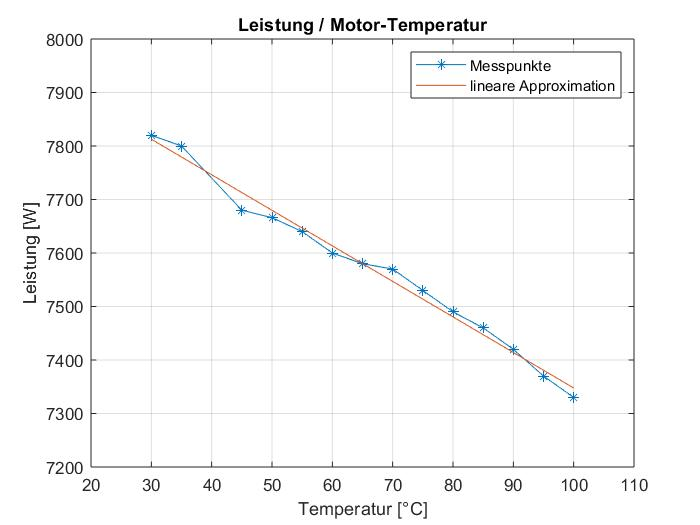
\includegraphics[width=1\linewidth]{LeistungTemperatur.jpg}
	\caption{Einfluss der Erwärmung auf die Leistung}\label{fig:Leistung/Temperatur}
\end{figure}

Wird in einem der nachfolgenden Versuche erwähnt, dass die Leistungs-Temperaturabhängigkeit berücksichtigt wurde, ist dies gleichbedeutend mit einer Temperaturskalierung aller Messwerte auf eine Temperatur von 70°C. Dies wird durch Einkalkulierung der in diesem Versuch ermittelte lineare Approximation erreicht, wodurch jeder einzelne Messwert schlussendlich dasselbe Temperaturniveau besitzt und somit die Messung temperaturunabhängig ist.